\newsection
\subsection{Robotics}
\label{sec:robotics}
\sectionauthors{Siddharth Karamcheti, Annie Chen, Suvir Mirchandani, Suraj Nair, Krishnan Srinivasan, Kyle Hsu, Jeannette Bohg, Dorsa Sadigh, Chelsea Finn}

\begin{figure}[!ht]
\centering
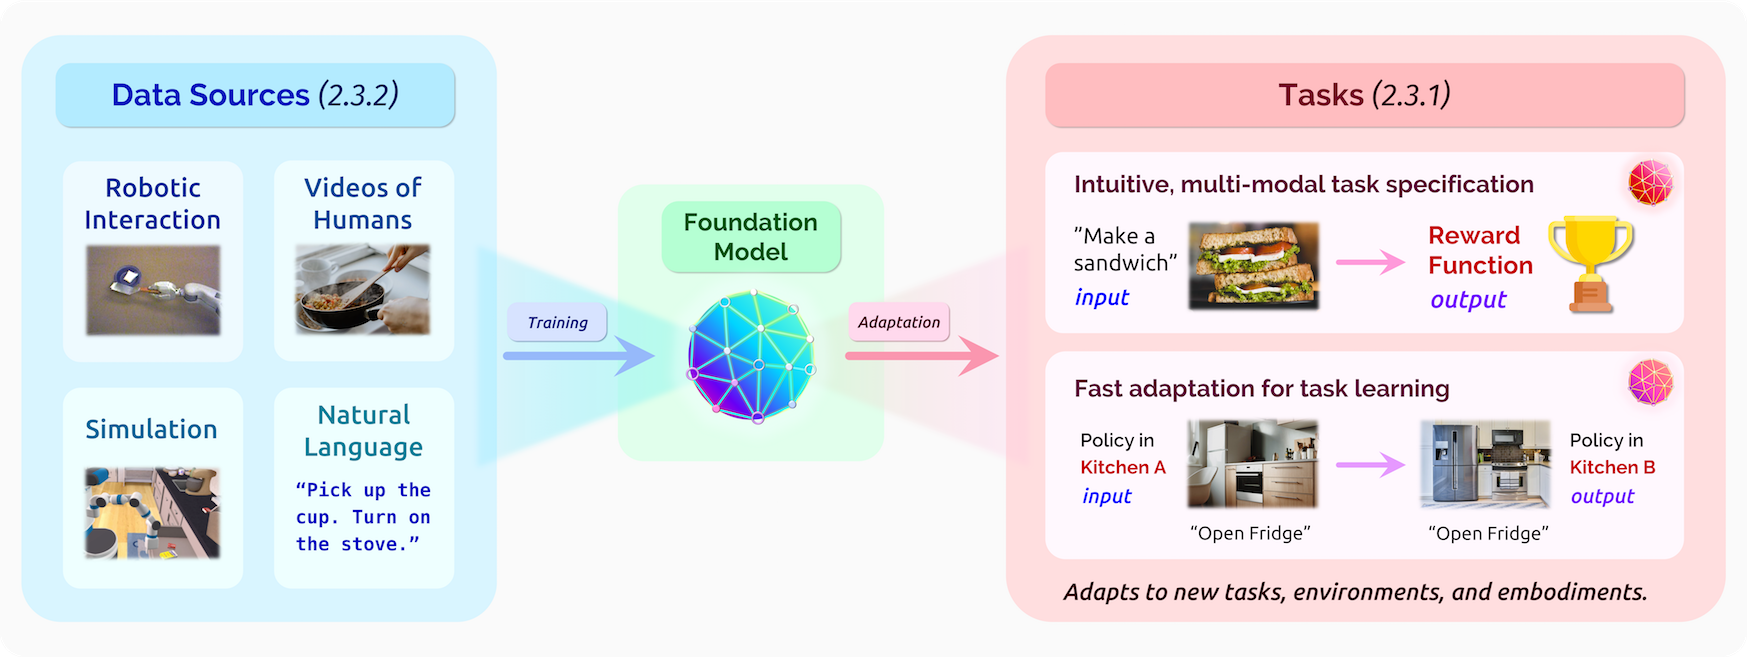
\includegraphics[width=\linewidth]{capabilities/figures/Robotics.png}
\caption{Foundation models for robotics require massive datasets spanning diverse environments and behaviors. Simulation, robotic interaction, videos of humans, and natural language descriptions could all be useful data sources for these models. Despite the challenges of acquiring data, foundation models for robotics have tremendous potential for a variety of problem formulations in task specification and robot learning. Image credits: \cite{finn2016deep, szot2021habitat}.}
\label{fig:robotics}
\end{figure}

\noindent 
A longstanding challenge of robotics research is to endow robots with the ability to handle the myriad conditions they will encounter in real-world settings. In this section, we discuss how foundation models can potentially help bring about ``generalist'' robots that can, for example, cook a new meal in a new house, with a new kitchen. We focus on the application of foundation models to the challenges of \textit{physical embodiment}\dash{}an axis that presents a stark contrast from problems traditionally studied in language and computer vision, where such models have already seen success. The promise of foundation models for robotics is in their ability to amplify the potential robots to improve key facets of daily life ranging from manufacturing \citep{nof1999handbook, sanneman2020state}, construction \citep{khoshnevis2004automated, bock2007construction}, autonomous driving \citep{thorpe1988vision, badue2020self}, to household aid \citep{thrun1995lifelong, brooks2002flesh, Dillmann2004TeachingAL, goodrich2007hri, Gupta2018RobotLI, shridhar2020alfred} and personal assistance \citep{dragan2013formalizing, javdani2018shared}, amongst others. Our discussion in this section primarily focuses on mobile manipulation robots for household tasks, but we expect its essence to be broadly applicable to the other use-cases of robotics listed above.

On the critical path towards foundation models for robotics is embracing opportunities in \textit{task specification} and \textit{task learning}, coupled with tackling challenges in \textit{data acquisition} and \textit{safety and robustness}. Consider the following robot learning paradigm: starting with a description of a task capturing what a user might like the robot to do (\eg ``make breakfast'')\dash{}learn a corresponding \textit{policy} to generate the desired robot actions. While policies can be parameterized in different ways, a common choice is that of a function that maps the task representation and environment observation (\eg a scene image from a fixed or egocentric camera, or inputs from alternative sensors like LIDAR) to robot actions \citep{andrychowicz2017hindsight, nair2018rig}. As the robot acts in a task-conditioned manner, the subsequent states are fed back to the policy, generating more actions until the task has been satisfied.

Yet, implementing such a paradigm in practice is difficult. To begin, what is the right interface for describing one's goals? For a given user in one context, ``make breakfast'' carries an implication of a full breakfast that consists of fried eggs, toast, and a glass of orange juice; for another user, ``make breakfast'' may imply idlis with sambar and a tumbler of filter coffee. In general, high-level context-dependent goals like these do not stand alone and can introduce a multitude of ambiguities. How does one \textit{specify} a goal (and corresponding subgoals) with enough clarity to both resolve these ambiguities, and in so doing, allow a robot to make progress on the given task? Additionally, how might we craft general task representations that might aid generalization to similar objectives (\eg fetching a glass of milk instead of orange juice). Going a step further, how do we build methods that aid robots in \textit{learning} policies for new tasks and new environments (in this case, a brand new kitchen with new utensils, appliances, layouts, etc.)?

Recent breakthroughs in applying foundation models for language and vision (\refsec{language} and \refsec{vision}) suggest several potential benefits these models have for improving generalization. The ability to tap into diverse streams of data to learn meaningful representational priors (akin to those learned by models such as BERT and GPT-3) holds promise for learning powerful foundation models for task specification; one could also use this data (following work in computer vision and video-processing) to bootstrap powerful foundation models for learning action-conditional dynamics models or policies indexing general and semantically meaningful skills. Yet while these opportunities exist, the key stumbling block is \textit{collecting the right data}. Unlike language and vision data, robotics data is neither plentiful nor representative of a sufficiently diverse array of embodiments, tasks, and environments\dash{}we (as a field) still have not converged on the \textit{type} of data that would be maximally useful for enabling generalist robotics (\eg offline demonstrations, third-person recordings of humans, egocentric videos, autonomous experience, etc.) Coupled with issues in obtaining the right scale and diversity of data are questions of ensuring safety and robustness: how do we behave in a new environment without causing damage?

The application of foundation models for robotics thus consists of a dichotomy of opportunities and challenges: opportunities for task specification and learning balanced against challenges of data collection and safe deployment. This section explores both by presenting a picture of how foundation models might help us develop generalist robots, in a way that not only meaningfully addresses the challenges associated with building such systems, but that also embraces the potential of multi-modality\dash{}incorporating perception, actuation, and language\dash{}as well as human-robot interaction for specification and learning.

\subsubsection{Opportunities}
\label{sec:robotics-opportunities}

Foundation models for robotics could take a variety of forms: problems in robotics do not easily conform to a one-size-fits-all model, since different problems have different input-output signatures\dash{}a contrast to domains like NLP where many problems can be cast into a general ``text-in, text-out'' signature. We focus on opportunities in generalizable task specification and learning across tasks, environments, and robot embodiments.

\paragraph{Foundation models for task specification.} Before robots can learn \textit{how} to solve tasks in a general purpose way, they must understand \textit{what} the desired task is: for example, to be useful in a new kitchen, a robot needs to know what we would like it to cook, as well as behaviors we would like it to avoid. Therefore, a necessary first step towards developing generalist robots is building models for reliable \textit{task specification}, \ie the intuitive and effective communication of task objectives, preferences, and constraints. We formalize task specification as a process that transforms a human-provided task description into a quantitative metric that measures a robot’s task completion and progress\dash{}\eg a reward function. This signal is crucial for optimizing robot behavior, diagnosing failures, and prompting human feedback. As the most natural way to describe a task can vary depending on the user, environment, or task, foundation models for task specification should accept a variety of description modalities, such as goal states \citep{fu2018variational, singh2019endtoend}, natural language \citep{macglashan2015grounding, karamcheti2017draggns, misra2017mapping, coreyes2019guiding, shao2020concept2robot}, videos of humans \citep{shao2020concept2robot, chen2021generalizable, liu2018imitation}, pairwise or ranking comparisons \citep{biyik2018batch}, interactive corrections \citep{coreyes2019guiding, karamcheti2020decomposition} and physical feedback \citep{ross2011reduction, bajcsy2017learning}.

An important requirement of general purpose models for task specification is the ability to transfer to \textit{new} environments and tasks. Reliably transforming task descriptions into generalizable reward signals for robot learning remains an open problem \citep{taylor2016alignment}\dash{}one that foundation models are well suited for. When applied to task specification, foundation models can provide more robust (\refsec{robustness}) general purpose reward signals by learning from large and broad datasets\dash{}even leveraging \textit{multiple} of description modalities listed above. One concrete instantiation of a foundation model for task specification might be a model that learns a mapping from arbitrary (language, current observation) pairs to reward signals by training on diverse language and vision datasets \citep{bahdanau2019reward, fu2019lang2goals, chen2021generalizable}. By learning informative priors from these broad, diverse datasets, such a model may be able to generalize to unseen language instructions and observations in unseen environments. In general, the ability of foundation models to deftly bridge modalities and generalize broadly make them attractive for general purpose task specification.

\paragraph{Foundation models for task learning.} In addition to enabling more general task specification, foundation models could make learning to solve new tasks more efficient and reliable. In this context, a foundation model for robotics might take the form of a joint distribution over actions, observations, rewards, and other properties of interest. Conditioning on different dimensions of this joint distribution recovers different inference problems, each corresponding to a different signature:
\begin{itemize} 
    \item \textit{Dynamics modeling}: $p$(future observations $\mid$ actions, past observations) \citep{finn2017deep, hafner2019latent, wu2021greedy}.
    \item \textit{Policy learning}: $p$(actions $\mid$ observations, goal) \citep{kaelbling1993learning, schaul2015uvf, ding2019goal}.
    \item \textit{Inverse reinforcement learning}: $p$(reward function $\mid$ observations, actions) \citep{ng2000algorithms, ziebart2008maximum, finn2016guided}.
\end{itemize}
To train on raw data from a diverse array of robots, foundation models operating on observations must account for the vast set of plausible sensor configurations and modalities. While seemingly a challenge, this actually presents an opportunity: cross-modal representations can be more general and grounded, leveraging arbitrary input configurations while taking advantage of correspondences between modalities \citep{kaiser2017one, li2019connecting, lee2020detect, lee2020multimodal, alayrac2020self, jaegle2021perceiver}. Self-supervision presents an additional opportunity: one plausible training objective for a foundation model for robotics is to predict the different elements of the joint distribution described above in an autoregressive fashion  \citep[][\refsec{modeling}]{Janner2021ReinforcementLA, Chen2021DecisionTR}. This objective could allow foundation models to tap into unlabeled data\dash{}as long as the data exhibit diverse, meaningful behavior. \refsec{robotics-challenges} discusses the challenges of collecting such data further.

In language and vision, foundation models have demonstrated the capability to learn broadly applicable priors from large, diverse datasets, that can be subsequently adapted to downstream tasks (\refsec{language}, \refsec{vision}). Foundation models for robotics have the potential to similarly enable few-shot adaptation of perception and control to new environments, tasks, and embodiments. Consider our running kitchen example. To cook in a new kitchen, a robot needs to adapt to the specific environment\dash{}its spatial layout, the available equipment, etc. Priors learned from offline videos of humans, robotic interaction, text, and/or simulation (\refsec{robotics-challenges}) might encode general aspects of kitchens, such as the fact that stoves are usually against walls and must be turned on in order to produce heat. Such commonsense knowledge, physical priors, and visual priors could make adaptation to new environments more sample efficient. Similarly, a foundation model for robot task learning might be able to use a large number of cooking videos in its training dataset to adapt a policy for a common skill, such as ``fry an egg,'' to a specific user’s preferences from a low number of demonstrations\dash{}allowing for sample efficient adaptation. Finally, with their potential to learn the cross-modal representations described earlier, foundation models for robotics could help enable adaptation to new embodiments. This aspect of adaptation is crucial to make these models widely useful.

\subsubsection{Challenges and risks}
\label{sec:robotics-challenges}

Despite this exciting vision, multiple challenges need to be overcome. To enable the generalization discussed above, we must collect robotic datasets of sufficient size and diversity. Additionally, we need mechanisms to ensure that we can deploy learned behaviors safely in the real world.

\paragraph{Data needs \& challenges.} Learning a policy for a robot that perceives the state of its environment via sensors and takes actions to accomplish tasks traditionally requires large datasets of the robot \textit{interacting in the real world}. On the other hand, many learning tasks in computer vision and natural language processing rely on large and diverse \emph{offline} datasets that can easily be scraped from the web. Motivated by the advances of foundation models in language and vision, we are excited by the possibility of leveraging large offline data sources for learning such models in robotics.

One path towards this goal is collecting large datasets for offline learning, for example using teleoperation \citep{mandelkar2019scaling}, kinesthetic teaching \citep{sharma2018mime}, or autonomous methods \citep{pinto2016supersizing, Gupta2018RobotLI, Levine2018LearningHC, dasari2019robonet, kalashnikov2021mt}, which have shown some promising indications on generalization. While scaling up robot data collection to the size of vision and language datasets  \citep{deng2009imagenet, krishna2017visual, raffel2019exploring, gao2020pile} remains an open challenge, the increasing scale and quality of robotic datasets suggests they can play an important role in learning foundation models for robotics. 

Given the challenging closed-loop nature of learning control, it is possible that collecting such datasets of size comparable to those used in vision and language is insufficient for robotics. One exciting option is to additionally leverage external, non-robotic sources of data such as videos of humans or existing vision and natural language datasets. Such data is diverse and exists in large quantities on the web \citep{deng2009imagenet,Lee2012DiscoveringIP, caba2015activitynet, Goyal2017TheS, damen2018kitchens, gao2020pile}, affording the possibility of broad generalization if properly leveraged. Elegantly addressing the gap between the robot’s domain and those found in videos or language on the web remains an open challenge; however, recent progress in domain adaptation \citep{Smith2019AVIDLM, Schmeckpeper2020ReinforcementLW} and using pretrained video and language models in robotics \citep{lynch2020grounding, shao2020concept2robot, chen2021generalizable} present promising directions towards closing this gap.

Finally, simulation presents a boundless source of rich interactive data that robots can learn from, with a range of sensor modalities like rendered visuals, point-clouds, and simulated touch/audio. However, a major challenge lies in bridging the gap between simulation and the real world, both in the underlying physics and in the semantic distribution of environments and tasks. Recent work has shown that by using extensive domain randomization, tasks ranging from flight \citep{Sadeghi2017CAD2RLRS} to contact-rich manipulation \citep{Mahler2017DexNet2D, OpenAI2019SolvingRC} and locomotion \citep{RoboImitationPeng20, hwangbo2019learning} skills learned in simulation can be transferred to real robots with some success, and that the semantic and visual distribution of the real world can be simulated by scanning the real world into a simulation \citep{Matterport3D, Kolve2017AI2THORAI, embodied, szot2021habitat, shen2021igibson}. While these are promising steps towards closing the sim-to-real gap, effective and general sim-to-real learning of manipulation and locomotion skills remains an open challenge. Simulation data, real robot data, videos of humans, and natural language data could all be essential to learning foundation models for robotics.

\paragraph{Safety \& robustness.} Further complicating the development of foundation models for robotics is ensuring their safety and robustness when training or deploying them in the real world. We can expect the safety risks from these models for robotics to be different from their language counterparts given that embodied agents are empowered to manipulate and interact with their surroundings directly in the physical world while collecting data. One core safety challenge for learning-based systems is the chicken-and-egg problem of needing to specify system constraints for safety prior to collecting data, after which unforeseen unsafe behaviors requiring additional constraints may emerge. For instance, an agent adapting to a new kitchen outside of the training distribution requires sufficient safety guarantees to ensure safe data collection, which may either adversely affect task performance or cause the agent to fail in novel ways. One way to resolve this is restricting the complexity of the environment or increasing the complexity of the robot such that irrecoverable states or unsafe actions are avoided by construction. The robot can also be tasked with autonomously resetting the environment to facilitate uninterrupted learning (or adaptation) from large-scale data collection \citep{eysenbach2017leave, gupta2021reset}. This would either mean ensuring that nothing in the kitchen is breakable, or ensuring and replacing the items the agent may break while it attempts to collect data.

To address risks posed by foundation models that fail to generalize or produce unexpected behaviors to new stimuli, potential future directions include developing a causal analysis of agents \citep{deletang2021causal}, new formal safety evaluation tools, and realistic simulation environments \citep{corso2020survey, dreossi2017compositional, Julian_2019}. Finally, deriving formal safety guarantees for foundation models, \eg Hamilton-Jacobi reachability of safe-sets \citep{chow2018lyapunov, fisac2019bridging, herbert2021scalable} or by developing safety boundaries for learning that are interpretable (\refsec{interpretability}) to human operators, could help reduce risks posed by foundation models for robotics \citep{berkenkamp2017safe}. As the study and implementation of foundation models progresses and intersects with robotics, solutions to these challenges will be crucial.

\paragraph{Conclusion.} While the promise of foundation models for robotics are many\dash{}spanning multiple levels of the robotics pipeline from task specification to task learning\dash{}the challenges are significant. Collecting data \textit{in the physical world} that covers diverse environments and embodiments at scale is a sizable hurdle, and ensuring the safety and robustness of such systems is equally exigent. Despite this, our optimism prevails; tackling these challenges now, \textit{before} developing models offers us the chance to identify ways to collect the right data, from the right sources, at the right scale to build safe and reliable foundation models with the capabilities we desire. 

Underpinning this section has been a theme of multimodality. Foundation models for robotics\dash{}in all possible instantiations\dash{}have and will continue to benefit from work in other subfields of AI such as language and vision (\refsec{language}, \refsec{vision}). Yet as we consider incorporating these extensions from other fields, there are interdisciplinary challenges on the horizon that touch other aspects of foundation models: systems innovation for training \textit{and deploying} such models for real-time robotics (\refsec{systems}), innovation in interfaces for robust human-robot interaction (\refsec{interaction}), and lessons to incorporate as we better grasp the safety and robustness of such models (\refsec{ai-safety}, \refsec{robustness}). Building a reliable ecosystem and thoughtful research practices around foundation models is key to realizing these goals.




